%!TEX TS-program = xelatex

% Официальный шаблон презентации НИУ ВШЭ в beamer (LaTeX)
% Версия 2.0
% Язык — русский

\documentclass[aspectratio=169]{beamer}

\newbool{russian}
\booltrue{russian}
\usepackage{HSE-theme/beamerthemeHSE}

%%% Работа с русским языком и шрифтами
\usepackage{multirow}
\usepackage{listings} 
\usepackage[dvipsnames]{xcolor}
\usepackage[english,russian,shorthands=off]{babel}
\usepackage[no-math]{fontspec}
\usepackage{makecell}
	\IfFontExistsTF{HSE Sans}
		{\newcommand{\presentationfont}{HSE Sans}}
		{\newcommand{\presentationfont}{Arial}}
	\setsansfont{\presentationfont}
	\setmonofont{Courier New}

\usepackage[most]{tcolorbox}

\usepackage{mathspec}
	\setmathsfont(Digits,Latin,Greek)[Numbers={Lining,Proportional}]{\presentationfont}
	\setmathrm[Numbers={Lining,Proportional}]{\presentationfont}
\uselanguage{russian}
\languagepath{russian}
\deftranslation[to=russian]{Theorem}{Теорема}
\deftranslation[to=russian]{Definition}{Определение}
\deftranslation[to=russian]{Definitions}{Определения}
\deftranslation[to=russian]{Corollary}{Следствие}
\deftranslation[to=russian]{Fact}{Факт}
\deftranslation[to=russian]{Example}{Пример}
\deftranslation[to=russian]{Examples}{Примеры}

\usepackage{booktabs}
\usepackage{array}
\graphicspath{{images/}}


\newcommand{\term}[1]{{\large\textcolor{HSEblue}{#1}}}
\newcommand{\cmd}[1]{\textcolor{HSEblue}{\texttt{#1}}}
\lstset{ 
    basicstyle=\color{HSEblue}\ttfamily\small,
    numbers=left,
    numberstyle=\color{HSEblue}\ttfamily\scriptsize,
    frame=single,
    columns=fullflexible,
    keepspaces=true,
    showstringspaces=false,
    breaklines=true,
    rulecolor=\color{HSEblue},
}


%% Информация об авторе и выступлении

\title[Мобильные колесные роботы]{Оценка состояния робота и локализация по известной карте}
\subtitle{Проектный семинар <<Мобильные колесные роботы>>}
\author[Команда курса]{Дергачев Степан  Алексеевич, \texttt{\href{mailto:sadergachev@hse.ru}{sadergachev@hse.ru}} \\ Муравьев Кирилл Федорович, \texttt{\href{mailto:kmuravev@hse.ru}{kmuravev@hse.ru}}}
\institute{Факультет компьютерных наук НИУ ВШЭ}
\date{22 октября 2026}


% Заглушки иллюстраций: заменить вызов на includegraphics при добавлении рисунков.
\newcommand{\imageplaceholder}[2][3.4cm]{%
  \begingroup
  \setlength{\fboxsep}{7pt}%
  \setlength{\fboxrule}{0.4pt}%
  \fcolorbox{HSEblue!35}{white}{%
    \begin{minipage}[c][#1][c]{\dimexpr\linewidth-2\fboxsep-2\fboxrule\relax}
      \centering\small\color{HSEblue!65}#2
    \end{minipage}}%
  \endgroup
}

% Отключаем активные кавычки babel для совместимости с mathspec.
\AtBeginDocument{\shorthandoff{"}}
% Убираем лишний пробел после полноширинного блока номера страницы.
% Внешний вид и файл темы HSE остаются прежними.
\makeatletter
\patchcmd{\beamer@@tmpl@footline}{\end{beamercolorbox} }{\end{beamercolorbox}}{}{}
\makeatother
\begin{document}
\frame[plain]{\titlepage}

\section{Оценка состояния и датчики}

\begin{frame}
\frametitle{Задача оценки состояния}
\small
\begin{itemize}
  \item По информации о среде, данным с датчиков (измерениям), выбранным управлениям и модели движения требуется оценить состояние робота и неопределённость оценки.
  \item Состояние может включать положение, ориентацию, скорости и т.д.:
  \[ \mathbf x=(p_x,p_y,\theta,v,\omega, \ldots). \]
  \item Без информации о среде (карты) можно оценивать перемещение относительно начальной позы.
\end{itemize}
\end{frame}

\begin{frame}
\frametitle{Задача оценки состояния (вероятностная постановка)}
\small
\begin{columns}[T]
\column{0.48\textwidth}
\begin{block}{Дано}
\begin{itemize}
  \item Модели движения и измерений.
  \item Оценка начального состояния $p(\mathbf x_0)$.
  \item История управлений $\mathbf u_{0:k-1}$.
  \item История измерений $\mathbf z_{0:k}$.
  \item Информация о среде $m$ (если используется).
\end{itemize}
\end{block}
\column{0.48\textwidth}
\begin{block}{Определить}
Распределение текущего состояния:
\[
 p(\mathbf x_t\mid\mathbf \mathbf x_0, z_{0:k},\mathbf u_{0:k-1}, m).
\]
\end{block}
\end{columns}
\end{frame}

\begin{frame}
\frametitle{Датчики мобильного робота}
\begin{columns}[T]
\column{0.6\textwidth}
\small
\begin{itemize}
  \item \textcolor{HSEblue}{Энкодеры}: углы поворота и скорости вращения колёс.
  \item \textcolor{HSEblue}{IMU}: угловые скорости (гироскоп) и линейные ускорения (акселерометр). Опционально: угол относительно магнитного поля земли (магнитометр).
  \item \textcolor{HSEblue}{LiDAR и датчики расстояния}: расстояния до объектов в определенном направлении.
  \item \textcolor{HSEblue}{Камеры}: цвет для каждого пикселя.
  \item \textcolor{HSEblue}{Камеры глубины}: расстояние и цвет для каждого пикселя (RGB-D)
  \item \textcolor{HSEblue}{UWB}: расстояния между передатчиками.
\end{itemize}
\column{0.35\textwidth}
\vfill
\begin{center}
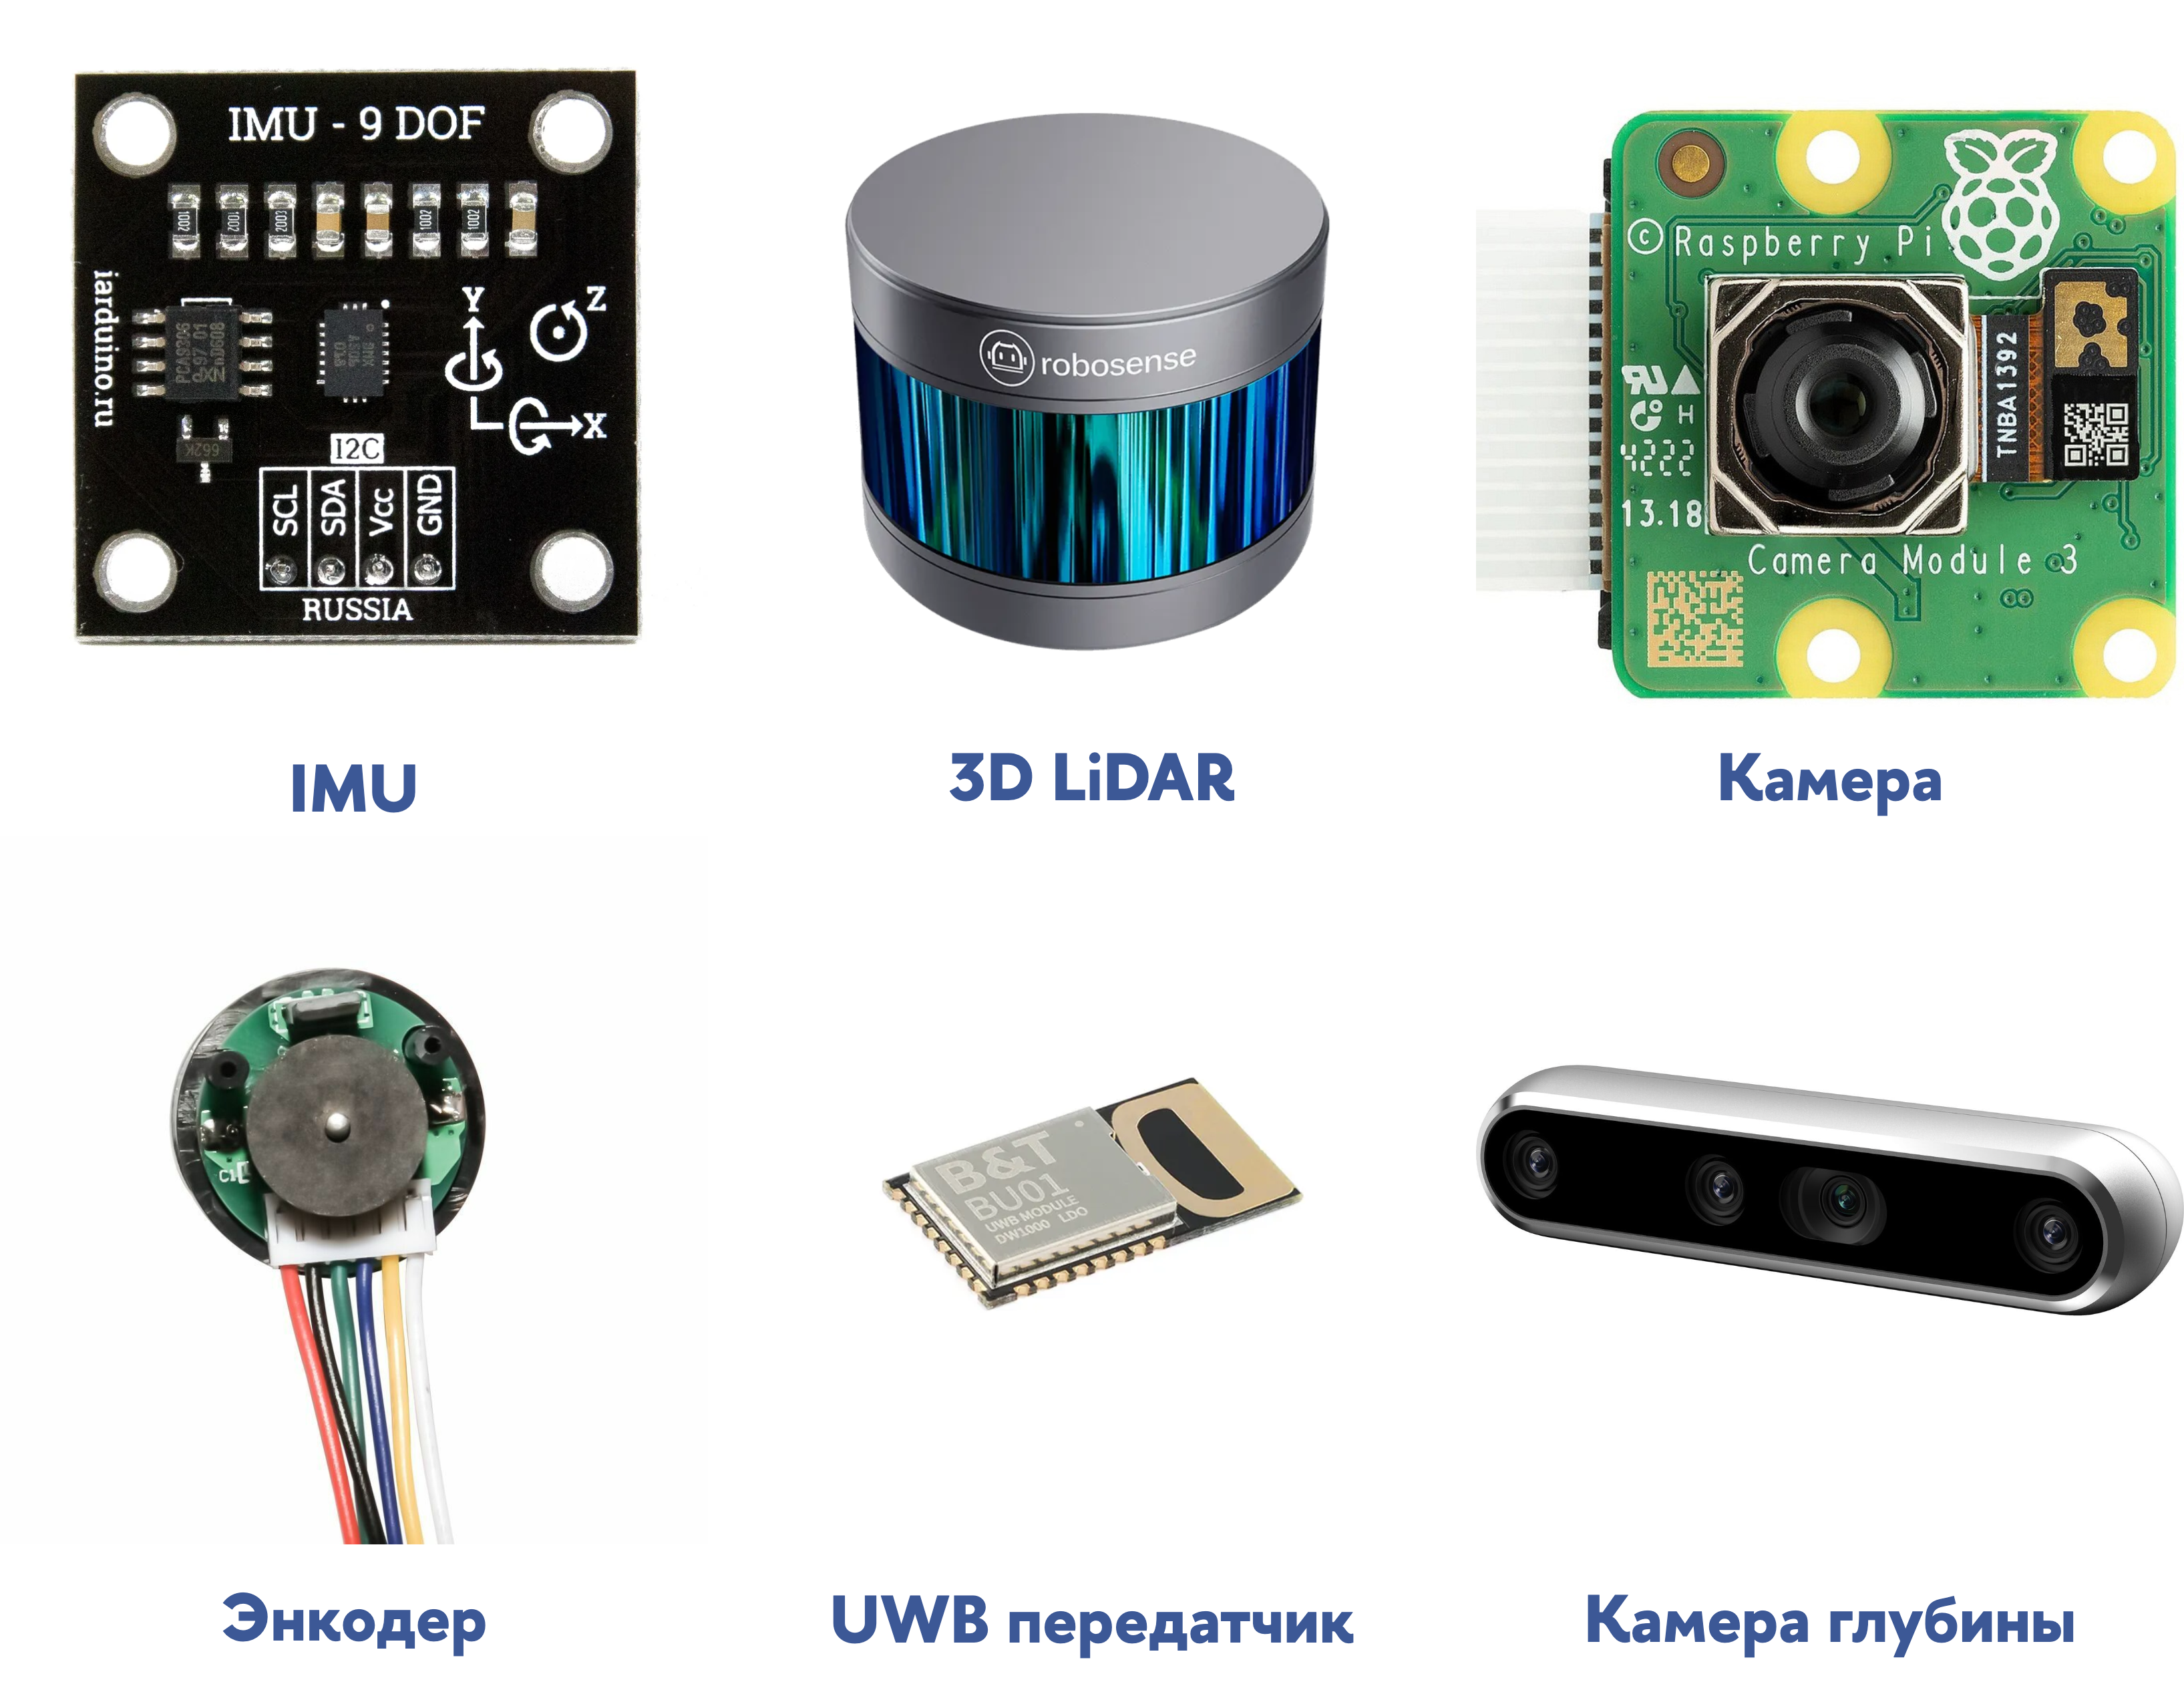
\includegraphics[width=0.99\columnwidth]{images/sensors.png}
\end{center}
\vfill
\end{columns}
\end{frame}

\begin{frame}
\frametitle{Одометрия и накопление ошибок}
\small
\begin{itemize}
  \item Накопление приращений движения даёт траекторию относительно начальной позы.
  \item Колёсная, инерциальная, визуальная и лидарная одометрия подвержены ошибкам.
  \item Ошибки накапливаются.
  \item Объединение нескольких источников может улучшить оценку состояния.
\end{itemize}
\end{frame}

\begin{frame}
\frametitle{Модель движения и модель измерений}
\small
\begin{block}{Модель движения}
\[
 \mathbf x_t=f(\mathbf x_{t-1},\mathbf u_{t-1})+\mathbf w_{t-1}.
\]
\end{block}
\begin{block}{Модель измерений}
\[
 \mathbf z_t=h(\mathbf x_t)+\mathbf v_t.
\]
\end{block}
\begin{itemize}
  \item $\mathbf w$ -- ошибка перехода, $\mathbf v$ -- ошибка измерения.
  \item Модель измерений также может учитывать управление и карту.
  \item Распределение шума -- допущение модели.
\end{itemize}
\end{frame}

\section{Фильтр Калмана}

\begin{frame}
\frametitle{Фильтр Калмана: модель и предположения}
\small
\begin{block}{Линейные модели движения и измерений}
\[
 \mathbf x_t=A\mathbf x_{t-1}+B\mathbf u_{t-1}+\mathbf w_{t-1},
 \qquad \mathbf z_t=H\mathbf x_t+\mathbf v_t.
\]
\end{block}
\begin{itemize}
  \item Начальное распределение состояния -- нормальное.
  \item Шумы независимы, имеют нормальное распределение и нулевое среднее:
  \[
  \mathbf w_{t-1}\sim\mathcal N(0,Q),\qquad
  \mathbf v_t\sim\mathcal N(0,R).
  \]
  \item $Q$ описывает неопределённость перехода, $R$ -- измерений.
  \item   При выполнении предположений фильтр минимизирует среднюю квадратичную ошибку оценки.
\end{itemize}
\end{frame}

\begin{frame}
\frametitle{Фильтр Калмана: представление оценки}
\begin{columns}[T]
\column{0.58\textwidth}
\small
\[
 \mathbf x\sim\mathcal N(\hat{\mathbf x},P).
\]
\begin{itemize}
  \item Среднее $\hat{\mathbf x}$ задаёт оценку состояния.
  \item Ковариация $P$ описывает неопределённость этой оценки.
  \item Диагональные элементы -- дисперсии отдельных компонент.
  \item Внедиагональные элементы описывают взаимосвязь ошибок компонент.
\end{itemize}
\column{0.38\textwidth}
\vfill
\begin{center}
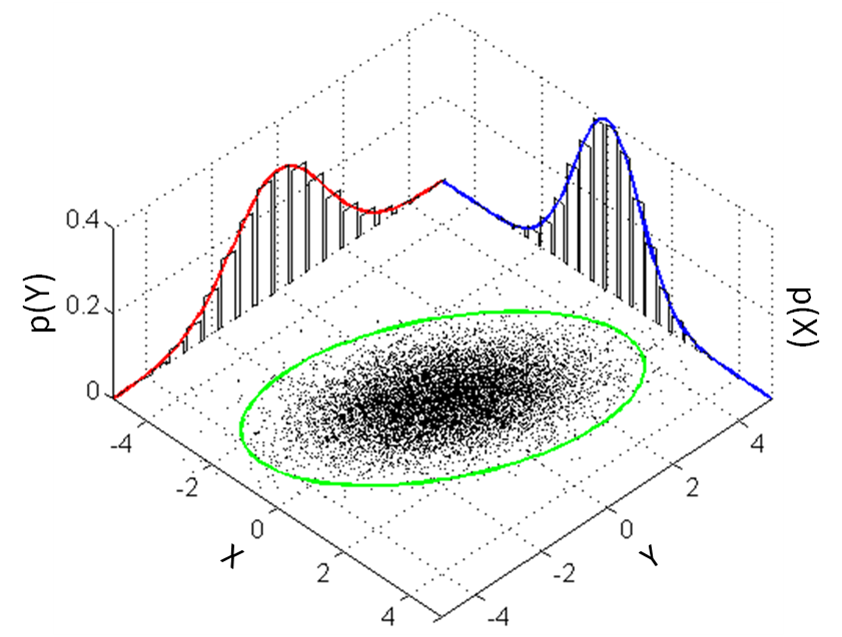
\includegraphics[width=0.99\columnwidth]{images/normal.png}
\end{center}
\vfill
\end{columns}
\end{frame}

\begin{frame}
\frametitle{Фильтр Калмана}
\small
\begin{block}{Предсказание}
По модели движения вычисляем новое состояние $\hat{\mathbf x}_{t, exp}$ и его неопределённость $P_{t, exp} = AP_tA^T+Q$.
\end{block}
\begin{block}{Коррекция}
\begin{itemize}
  \item Сравниваем измерение с ожидаемым : $\mathbf z_t-H\,\hat{\mathbf x}_{t,exp}$.
  \item Вычисляем коэффициент Калмана (степень доверия к предсказанию и измерению)
  \[K = \Sigma_0 (\Sigma_0 + \Sigma_1)^{-1}, \quad \Sigma_0 = HP_{t,exp}H^T,\; \Sigma_1 = R\]
  \item Корректируем оценку:
    \[H\hat{\mathbf x}_t = H\hat{\mathbf x}_{t, exp} + K(z_t-H\hat{\mathbf x}_{t,exp}), \quad HP_{t}H^T = HP_{t,exp}H^T - K \cdot HP_{t,exp}H^T\]
\end{itemize}
\end{block}
\end{frame}

\begin{frame}
\frametitle{Нелинейные модели}
\small
\begin{itemize}
  \item Модели движения и измерений могут быть нелинейными.
  \item Например, у колёсного робота перемещение нелинейно зависит от угла:
\end{itemize}
\[
 \begin{aligned}
 p_{x,t+1}&=p_{x,t}+v_t\cos\theta_t\,\Delta t,\\
 p_{y,t+1}&=p_{y,t}+v_t\sin\theta_t\,\Delta t.
 \end{aligned}
\]
\begin{itemize}
  \item После нелинейного преобразования распределение в общем случае перестаёт быть нормальным.
  \item Для оценки состояния используют приближённые методы: EKF и UKF.
\end{itemize}
\end{frame}

\begin{frame}
\frametitle{Нелинейные модели: EKF и UKF}
\small
\begin{columns}[T]
\column{0.48\textwidth}
\begin{block}{Расширенный фильтр Калмана\\(EKF)}
Прогноз по нелинейной модели. Для переноса ковариации -- линеаризация модели.
\end{block}
\column{0.48\textwidth}
\begin{block}{Сигма-точечный фильтр Калмана\\(UKF)}
Генерируются (сигма-)точки и пропускаются через модель. По результату вычисляются новые среднее и ковариация.
\end{block}
\end{columns}
\end{frame}

\begin{frame}
\frametitle{Пример: объединение энкодеров и IMU}
\begin{columns}[T]
\column{0.60\textwidth}
\small
\begin{itemize}
  \item Состояние: $\mathbf x=(p_x,p_y,\theta,v,\omega)$.
  \item Прогноз по текущим оценкам скоростей $v, \omega$
  \item  Энкодеры дают оценки линейной и угловой скорости: $(v_{\mathrm{enc}},\omega_{\mathrm{enc}})$.
  \item Гироскоп измеряет угловую скорость $\omega_{\mathrm{gyro}}$.
  \item При поступлении измерения прогнозируем состояние к его времени и выполняем коррекцию.
  \item Уточнённые скорости улучшают дальнейшую оценку перемещения.
  \item Модель нелинейна: используем EKF или UKF.
\end{itemize}
\column{0.36\textwidth}
\vfill
\begin{center}
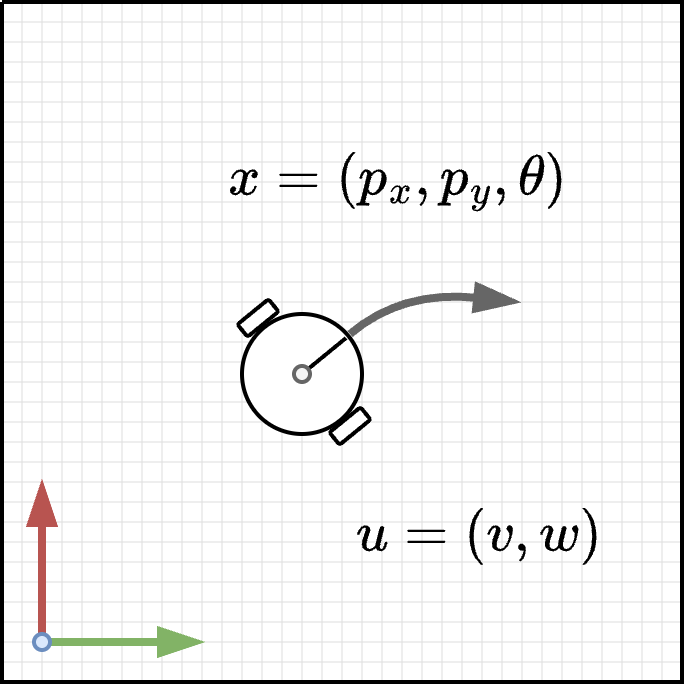
\includegraphics[width=0.99\columnwidth]{images/dd_vel.png}
\end{center}
\vfill
\end{columns}

\end{frame}



\section{Локализация по известной карте}

\begin{frame}
\frametitle{Локализация по известной карте}
\begin{columns}[T]
\column{0.62\textwidth}
\small
\begin{itemize}
  \item Локализация -- оценка позы робота в системе координат карты: $\mathbf x=(p_x,p_y,\theta)$.
  \item Частный случай задачи оценки состояния
  \item Доступна информаци о среде -- карта $m$.
  \item Доступно наблюдение среды $\mathbf z_{1:k}$ и информация об  движении $\mathbf u_{0:k-1}$.
  \item Требуется оценить: $p(\mathbf x_t\mid\mathbf z_{0:k},\mathbf u_{0:k-1},m)$.
\item Разделяют задачи:
  \begin{itemize}
    \item локальная локализация
    \item глобалная локализация
    \item задача "похищенного" робота
  \end{itemize}
  \end{itemize}
\column{0.34\textwidth}
\vfill
\begin{center}
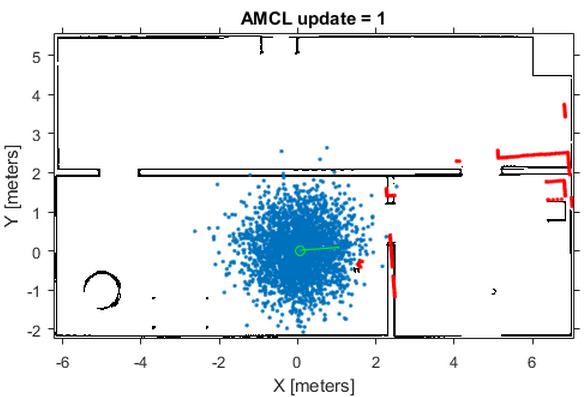
\includegraphics[width=0.99\columnwidth]{images/amcl_2.png}
\end{center}
\vfill
\end{columns}
\end{frame}

\begin{frame}
\frametitle{Пример представления среды}
\begin{columns}[T]
\column{0.45\textwidth}
\small
\begin{itemize}
  \item \textcolor{HSEblue}{Карта занятости (occupancy grid)} -- дискретное представление пространства в виде сетки ячеек
  \item Каждая ячейка хранит информацию о наличии препятствия (занято/свободно/неизвестно).
  \end{itemize}
\column{0.50\textwidth}
\vfill
\begin{center}
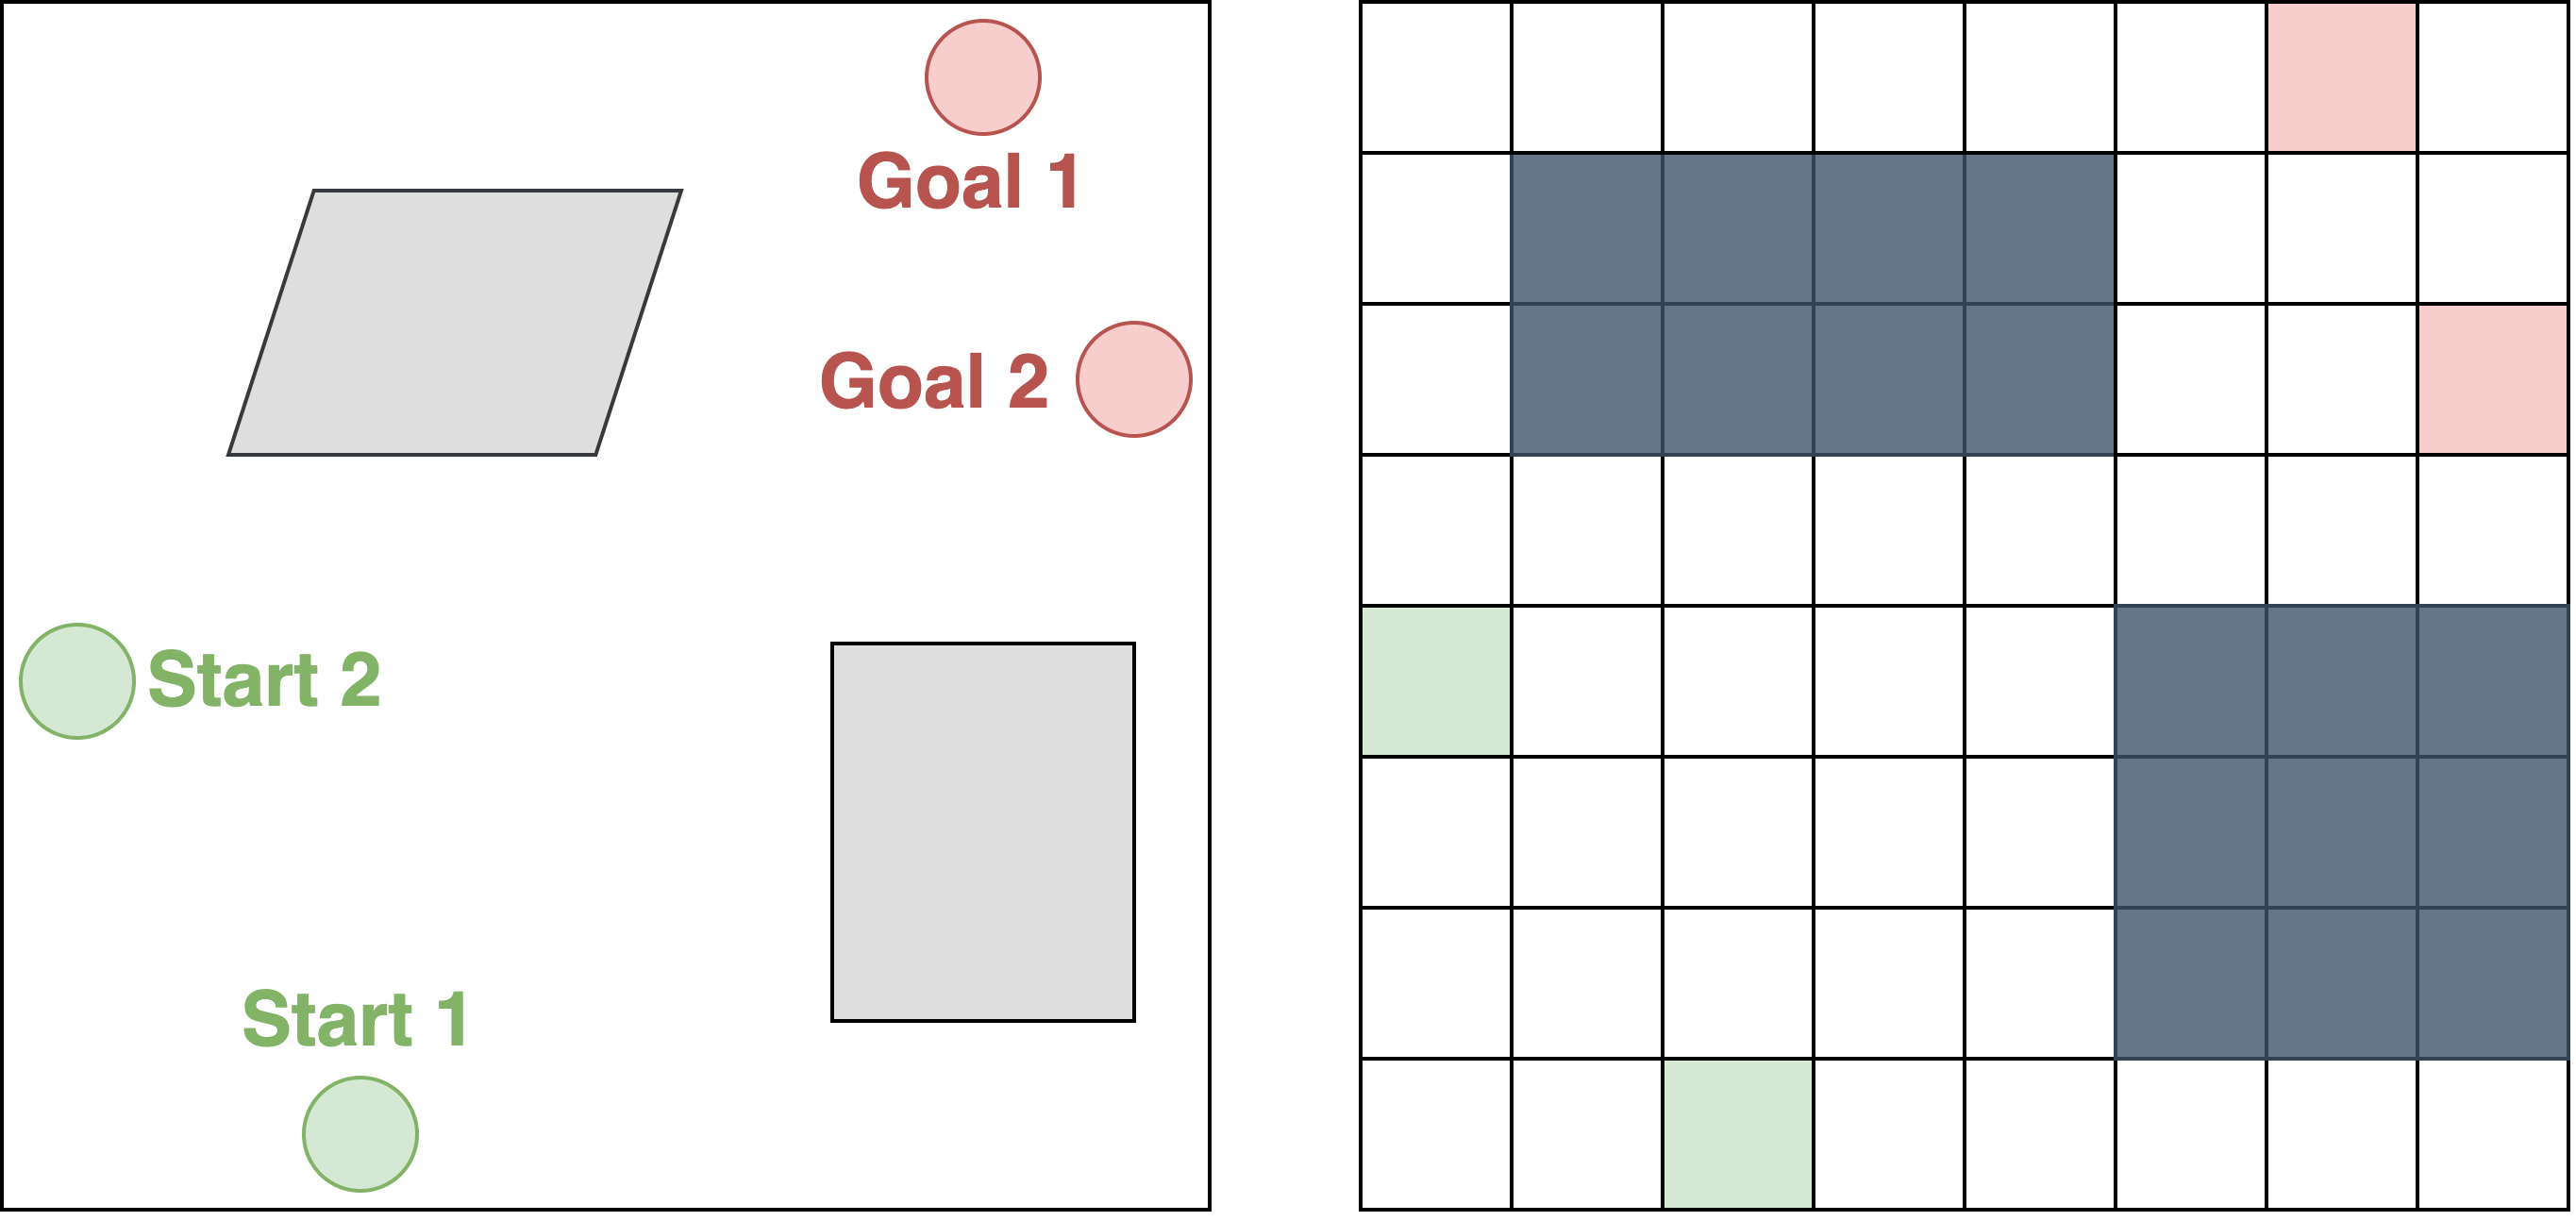
\includegraphics[width=0.99\columnwidth]{images/map.png}
\end{center}
\vfill
\end{columns}
\end{frame}


\begin{frame}
\frametitle{Фильтр частиц}
\begin{columns}[T]
\column{0.58\textwidth}
\small
\begin{itemize}
  \item Частица -- гипотеза позы робота:
  \[ \mathbf x^{(i)}=(p_x^{(i)},p_y^{(i)},\theta^{(i)}). \]
  \item Вес $w^{(i)}$ характеризует значимость гипотезы, $\sum_i w^{(i)}=1$.
  \item Частицы задаются около начальной оценки или по свободной области всей карты.
\end{itemize}
\column{0.38\textwidth}
\vfill
\begin{center}
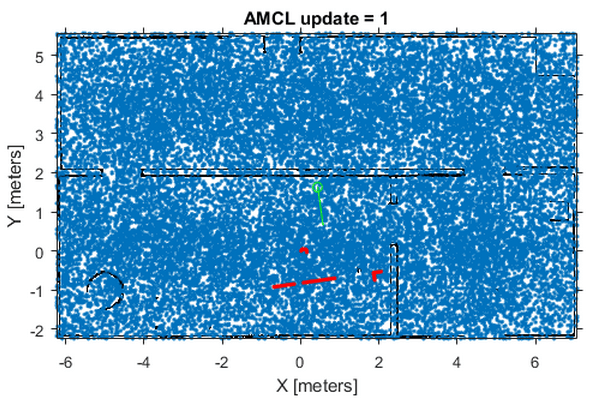
\includegraphics[width=0.99\columnwidth]{images/amcl_1.png}
\end{center}
\vfill
\end{columns}
\end{frame}

\begin{frame}
\frametitle{Фильтр частиц: прогноз}
\small
\begin{itemize}
  \item Получаем информацию о движении по одометрии.
  \item Перемещаем каждую частицу согласно модели движения.
  \item Добавляем случайную ошибку, учитывая неопределённость одометрии.
  \item Получаем новое облако гипотез.
\end{itemize}
\end{frame}

\begin{frame}
\frametitle{Фильтр частиц: обновление весов}
\small
\begin{itemize}
  \item Для каждой частицы оцениваем согласованность показаний датчиков (например скана LiDAR) с картой (например, картой занятости).
  \item Модель измерений задаёт правдоподобие $p(\mathbf z_t\mid\mathbf x_t^{(i)},m)$.
  \item Умножаем предыдущий вес на правдоподобие и нормируем веса.
\end{itemize}
\end{frame}

\begin{frame}
\frametitle{Фильтр частиц: ресэмплинг}
\small
\begin{itemize}
  \item Семплируем новый набор частиц с вероятностями, пропорциональными весам.
  \item Частицы с большими весами получают большое число новых "соседей", маловероятные гипотезы исчезают.
  \item Повторяем прогноз, обновление весов и ресэмплинг.
\end{itemize}
\end{frame}

\begin{frame}
\frametitle{Фильтр частиц}
\vfill
\begin{center}
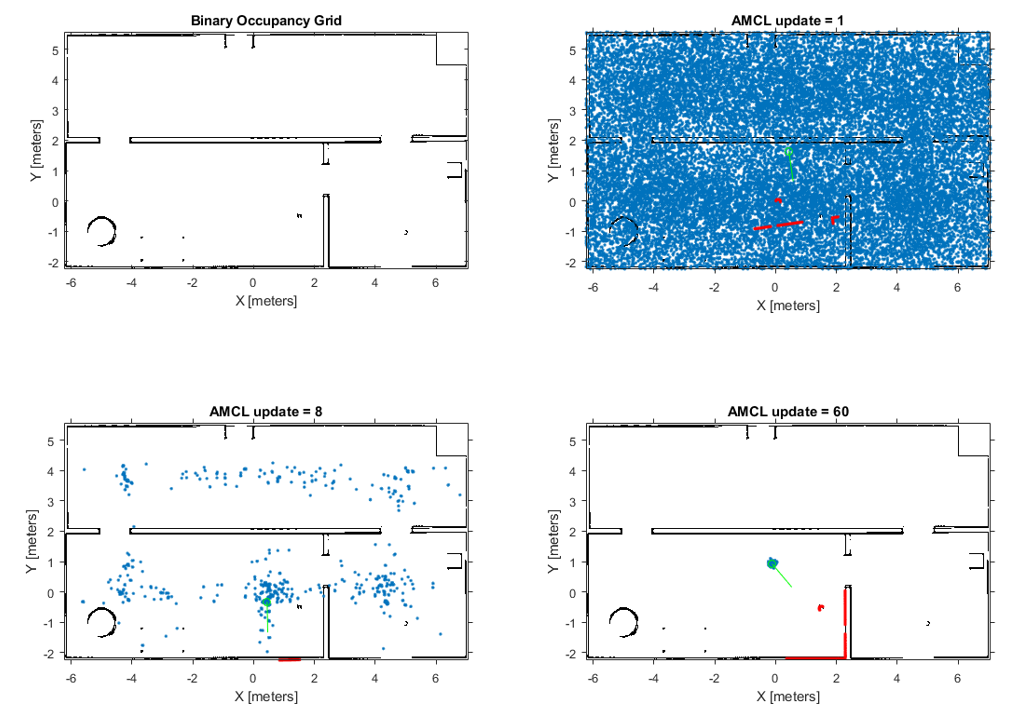
\includegraphics[height=0.99\textheight]{images/amcl.png}
\end{center}
\vfill
\end{frame}

\section{Оценка состояния в ROS2}

\begin{frame}
\frametitle{Оценка состояния и локализация в ROS2}
\small
\begin{block}{Пакет \cmd{robot\_localization}}
Повышение точности одометрии путем объединения измерений на основе EKF или UKF. Задает преобразование систем координат:
\[
 \texttt{odom}\to\texttt{base\_link}.
\]
\end{block}
\begin{block}{Пакет AMCL (Nav2)}
Локализация по карте. Задает преобразование систем координат::
\[
 \texttt{map}\to\texttt{odom}.
\]
\end{block}
\end{frame}

\begin{frame}
\frametitle{Локализация AMCL}
\small
\begin{itemize}
  \item Входные данные: известная карта занятости, сканы 2D LiDAR и одометрия.
  \item Необходимо преобразование между системами координат корпуса робота и LiDAR: \cmd{base\_link} $\to$ \cmd{laser}.
  \item Можно задать приблизительую начальную позу (например через \cmd{rviz} или \cmd{foxglove}).
  \item В режиме глобальной локализации при инициализации распределяет частицы по всей карте.
\end{itemize}
\end{frame}

\begin{frame}
\frametitle{Полезные материалы}
\small
\begin{itemize}

  \item  
  \href{https://github.com/literator1996/veroyatnostnaya_robototehnica/tree/master}{С. Трун, В. Бургард, Д. Фокс. Вероятностная робототехника (перевод на русский язык)}.
  \item\href{https://github.com/oleg-Shipitko/mipt_wheeled_robots_modeling_2022/blob/main/slides/Lecture\%202.\%20Localization.pdf}{Лекции О. Шипитко (МФТИ). Лекция 2. Локализация колесных роботов}.  
  \item \href{https://www.youtube.com/watch?v=NrzmH_yerBU&t=22s}{YouTube-канал MATLAB Tech Talk.  Understanding the Particle Filter (Визуализация фильтра частиц)}.
\end{itemize}
\end{frame}

\begin{frame}
\begin{center}
\Large Спасибо за внимание!
\end{center}
\vfill
\end{frame}

\end{document}
